\pdfinfoomitdate=1
\pdftrailerid{}
\pdfsuppressptexinfo=15
\documentclass[11pt]{article}
\usepackage[T1]{fontenc}
\usepackage{lmodern,microtype}
\usepackage[margin=1.04in]{geometry}
\usepackage{amsmath,amssymb,amsthm,mathtools,booktabs,array}
\usepackage{xcolor,tikz}
\usepackage[colorlinks=true,linkcolor=blue!45!black,citecolor=blue!45!black,urlcolor=blue!45!black]{hyperref}
\hypersetup{pdftitle={Single-fold Diophantine representations},pdfauthor={OpenAI}}
\newtheorem{theorem}{Theorem}[section]
\newtheorem{proposition}[theorem]{Proposition}
\newtheorem{lemma}[theorem]{Lemma}
\newtheorem{corollary}[theorem]{Corollary}
\theoremstyle{definition}
\newtheorem{definition}[theorem]{Definition}
\theoremstyle{remark}
\newtheorem{remark}[theorem]{Remark}
\newcommand{\NN}{\mathbb N}
\newcommand{\ZZ}{\mathbb Z}
\newcommand{\QQ}{\mathbb Q}
\newcommand{\Pow}{\operatorname{Pow}}
\newcommand{\bits}{\preccurlyeq}
\DeclareMathOperator{\rank}{rank}
\DeclareMathOperator{\im}{im}
\DeclareMathOperator{\sgn}{sgn}
\title{Single-fold Diophantine representations}
\author{OpenAI}
\date{September 24, 2026}
\begin{document}
\maketitle
\begin{abstract}
Every recursively enumerable set of natural-number tuples has a polynomial
Diophantine representation with exactly one complete auxiliary tuple for each
member. This proves the single-fold conjecture and, consequently, the finite-fold
conjecture.
\end{abstract}
\tableofcontents
\clearpage

\section{Introduction}
Throughout, $\NN=\{0,1,2,\ldots\}$. A set $S\subseteq\NN^n$ is
\emph{recursively enumerable} if a deterministic computation accepts exactly
its members; it may run forever on other inputs. A \emph{Diophantine
representation} of $S$ is a polynomial
\[
 P\in\ZZ[A_1,\ldots,A_n,W_1,\ldots,W_m]
\]
such that $a\in S$ if and only if $P(a,w)=0$ for some $w\in\NN^m$.
The representation is \emph{single-fold} if this complete tuple $w$ is unique
whenever it exists. It is \emph{finite-fold} if the set of such tuples is finite
for every input. These definitions count all auxiliary variables, including
those used to express subsidiary arithmetic operations.

\begin{theorem}\label{thm:main}
For every integer $n\ge1$ and every recursively enumerable set
$S\subseteq\NN^n$, there are an integer $m\ge1$ and a polynomial
$P\in\ZZ[A_1,\ldots,A_n,W_1,\ldots,W_m]$ such that, for every $a\in\NN^n$,
\[
 \#\{w\in\NN^m:P(a,w)=0\}=
 \begin{cases}1,&a\in S,\\0,&a\notin S.\end{cases}
\]
\end{theorem}

The Davis--Putnam--Robinson theorem established exponential Diophantine
representations of recursively enumerable relations: the defining expressions
may use exponentiation as well as addition and multiplication
\cite[Section~1]{dpr1961}. Robinson had shown how suitable growth conditions
yield an existential definition of exponentiation
\cite[Section~3]{robinson1952}. Matiyasevich's 1970 construction of an
exponentially growing Diophantine relation completed this route to polynomial
representations \cite[Sections~1 and~3]{mati1970}. The resulting representation
theorem implies the negative solution of Hilbert's tenth problem, since a
decision procedure for polynomial solvability would decide membership in every
recursively enumerable set. It does not bound the number of witnesses.

Matiyasevich obtained a different strengthening in 1974: every recursively
enumerable relation has an exponential representation with a unique complete
auxiliary tuple \cite[Section~2, Main Theorem]{mati1974}. The same paper
already formulates the remaining problem of polynomial representations with
this uniqueness and reduces it to single-fold binary exponentiation
\cite[Section~1]{mati1974}. This is the single-fold conjecture; allowing
finitely many witnesses gives the finite-fold conjecture \cite{mati2010}.
Theorem~\ref{thm:main} proves the single-fold assertion over $\NN$.
The witness domain matters: Miller and Shlapentokh obtain single-fold
definitions of computably enumerable sets of rational integers using
witnesses in characteristic-zero polynomial rings, and finite-fold definitions
of computably enumerable relations in polynomial rings over rings of
integers of totally real number fields \cite{millershlapentokh2022}.

Our arithmetic construction develops the classical strategy of recovering
powers from Pell solutions and controlling their indices through growth
bounds. Cantone, Cuzziol, and Omodeo give a recent account, including a
paired-Pell representation and the problem of replacing its exponential
cutoff \cite[Section~6, Lemma~6.1 and Theorem~5; Section~7]{cco2024}.
We supply a cutoff using rational points on a rank-one elliptic curve.
Poonen uses rank-one curves and denominator growth to obtain Diophantine
definitions between rings of integers
\cite[Theorem~1 and Section~2.3, Lemma~8]{poonen2002}.
Here the N\'eron--Tate height compares the full logarithmic x-coordinate
height with a quadratic function of an integer index, with uniformly bounded
additive error \cite[Chapter~VIII, Proposition~9.1 and Theorem~9.3]{silverman}.
The bounded additive error makes the exact index selection below possible.

The computational construction uses the bit-masking method of Jones and
Matiyasevich \cite{jm1984,jm1991}. Large-base encodings turn a finite
register-machine history into finitely many integers, and Lucas's binomial
congruence tests the permitted binary digits. Determining the base from the
input and computation time already appears in Chaitin's account
\cite[Sections~2.3 and~2.6]{chaitin1987}. We use a clock and a dyadic
interval to select one base for the entire run. Throughout both constructions,
uniqueness must include reduced rational coordinates, arithmetic quotients
and slacks, and the variables of inactive cases. The proof keeps this
complete-witness requirement through every substitution.

The arithmetic constants in the proof are fixed once for all sets $S$ and
all inputs. They include rational points and integers whose existence is
established below, but whose numerical values are not specified. The theorem
therefore gives existence of an integer polynomial without displaying its
coefficients or a procedure for numerically choosing those constants.

\begin{corollary}[Undecidability with an at-most-one-solution promise]
\label{cor:unique-h10}
There exist integers $m,D\ge1$ for which no algorithm has the following
property: on every input polynomial $F\in\ZZ[W_1,\ldots,W_m]$ of total
degree at most $D$ satisfying the promise
\[
 \#\{w\in\NN^m:F(w)=0\}\le1,
\]
the algorithm halts and correctly decides whether this set is nonempty.
\end{corollary}
The proof appears in Section~\ref{sec:consequences}, after the construction
of the single-fold representation.

\subsection{Proof overview}
The problem is to retain uniqueness when a computation is expressed by
polynomial equations. We first obtain unique arithmetic witnesses, then a
unique encoding of the accepting run. Section~\ref{sec:conventions} explains
how composition and disjoint cases preserve the complete witness, including
variables introduced inside subsidiary calls.

The arithmetic step begins with the rational points of
$E:y^2=x^3-25x$. Its group is $\ZZ P\oplus\mathcal T$, with $\mathcal T$
finite. Section~\ref{sec:elliptic} gives unique natural-number codes for
rational coordinates and point addition; Appendix~\ref{app:rank-one}
contains the rank calculation. Section~\ref{sec:growth} selects one point
for each positive absolute index $j=|n|$ among points $nP+t$, where
$n\in\ZZ$ and $t\in\mathcal T$. Apply a fixed scalar multiplication to
each selected point. Let $W_j$ be the maximum of the absolute reduced
numerator and positive denominator of its x-coordinate. These integer
heights satisfy
\[
 \log W_j=a_Ej^2+O(1),\qquad a_E>0,
\]
with a uniformly bounded error. The scalar can enlarge $a_E$ while leaving
that error bound fixed; a sufficiently large scalar also makes the sequence
strictly increasing.

A discrete difference of the quadratic main term makes exact index
selection possible. For positive indices $k,r$, the height product obeys
\[
 \log\frac{W_{2k}W_rW_1}{W_k^2W_{r+1}}
      =2a_E(k^2-r)+O(1).
\]
The error is bounded independently of both indices. A fixed multiplicative
window for the ratio therefore singles out $r=k^2$, once $a_E$ is large
enough to separate distinct integer values of $k^2-r$. The conditions use
only products, comparisons and fixed additions of rational points; the
indices and logarithms belong to their proof, not to the polynomial system.

For an input $u$, first choose the unique index $k$ with
$W_k\le u+W_1<W_{k+1}$, and then select the point at index $k^2$ by this
window. The output $g(u)=W_{k^2}$ has a single-fold graph. For large $u$, the quantity $k^2$ is comparable to $\log u$, and the
logarithm of the output is comparable to $(\log u)^2$. In particular, for some $\delta>0$ and all sufficiently
large $u$,
\[
 \delta(\log u)^2<\log g(u)<u\log u.
\]

Section~\ref{sec:power} uses these two bounds to select prescribed solutions
of two Pell equations. The upper bound forces their indices below a modulus,
so congruences determine those indices exactly. The lower bound ensures that
the intended solutions are admitted. An integer quotient then recovers
$c=b^n$, with a unique complete witness for every $b\ge2$ and $n\ge0$.
Section~\ref{sec:subset} uses powers and binomial parity to test whether
every nonzero binary digit of one integer is also nonzero in another.

Finally, Section~\ref{sec:computation} packs a deterministic counter
machine's states and counter values into digits of finitely many integers.
Binary containment restricts the permitted digits, and polynomial identities
enforce transitions and the first accepting halt. A clock fixes one
power-of-two base for the entire run. Thus every solution decodes to the
actual accepting computation, and that computation determines exactly one
complete tuple. Substituting the single-fold arithmetic systems and taking
a sum of squares proves Theorem~\ref{thm:main}.
Appendix~\ref{app:witnesses} specifies all coordinates counted in this
uniqueness assertion.

\section{Polynomial constructions with unique witnesses}\label{sec:conventions}
This section fixes the meaning of the polynomial notation used in the proof.
Its purpose is to make uniqueness survive every substitution, case distinction,
and auxiliary arithmetic operation.

\begin{definition}
A \emph{single-fold polynomial system} for a relation $R\subseteq\NN^d$ is a
finite list of integer polynomial equations $F_i(a,z)=0$ such that the set of
complete tuples $z$ is a singleton for $a\in R$ and empty otherwise.
A \emph{single-fold graph} of a function $f:D\to\NN^e$, where
$D\subseteq\NN^d$, is such a system for
$\{(a,f(a)):a\in D\}$. Thus each input $a\in D$ determines both the output and
all further auxiliary variables uniquely. Inputs outside $D$ have no solutions.
\end{definition}

All unspecified variables in polynomial systems range over $\NN$. Integer
polynomials may have negative coefficients. In particular, a displayed
inequality $F\ge G$ means $F-G=s$ with a new variable $s\in\NN$, and $F>G$
means $F-G=1+s$. The slack is unique; the values of $F$ and $G$ need not
separately be nonnegative. An integer $z$ is represented by its unique sign
code $z=z^+-z^-$, where $z^+,z^-\in\NN$ and $z^+z^-=0$.
Its absolute value is $z^++z^-$. Whenever a polynomial expression is passed as
a natural-number argument to a system, it can be replaced by a fresh variable
equal to that expression. This introduces a unique variable and enforces the
required nonnegativity.

The following closure operations belong to the single-fold constructions of
\cite[Sections~3.1--3.3]{mati1974}. In particular, disjoint alternatives require
fixing variables that are unused in the chosen case; see also
\cite[Section~2, pp.~590--591]{cco2024}. We state the precise version needed
here.

\begin{lemma}[Composition and disjoint cases]\label{lem:composition}
Finite conjunctions of single-fold polynomial systems, using separate
auxiliary tuples for distinct calls, preserve uniqueness for fixed values of
all their displayed arguments. Composition of single-fold graphs preserves
uniqueness of outputs and complete auxiliary tuples. A finite union of
single-fold relations also has a single-fold system if their displayed
argument sets are pairwise disjoint.
\end{lemma}
\begin{proof}
For conjunction, each auxiliary tuple is fixed by its call's arguments. In a
composition of functions, fix the first input and successively determine every
intermediate output and its auxiliary tuple. This proves both existence and
uniqueness along the chain.

For a disjoint union with $r$ cases, introduce selectors $e_1,\ldots,e_r$ with
\[
 e_i(e_i-1)=0,\qquad \sum_{i=1}^r e_i=1.
\]
Write every equation in case $i$, including its guard and all equations inside
nested calls, in the form $F=0$, and replace it by $e_iF=0$. For each variable
$z$ local to this case, also impose $(1-e_i)z=0$. This last rule applies to all
local coordinates, outputs of local calls, normalization variables, selectors,
and slacks, including those inside nested calls. Displayed arguments shared
between cases are not local variables. Exactly one selector equals one.
Its case has its unique witness tuple, while every other case has all local
variables zero. Disjointness makes the selector itself unique.
\end{proof}

When defining a function by cases, we additionally require the guards to
partition its input domain and each active case to determine the shared
output. This is the form used below.

For example, $h=\max(a,b)$ is obtained from the disjoint cases $a\ge b$, $h=a$
and $a<b$, $h=b$. The strict inequality in the second guard assigns ties to
one case. Quotient and remainder on division by a positive integer $d$ are
specified by $a=dq+r$ and $r<d$; both and the slack are unique.
No unbounded choice of a B\'ezout coefficient or of an inactive-case variable
is permitted in the constructions below.

Point coordinates will be given fixed tuples of natural numbers in
Section~\ref{sec:elliptic}. A single-fold system on such points always means a
system on these entire tuples. To use an unprescribed point existentially, its
entire code is part of the witness. We will prove uniqueness of that point
before appealing to uniqueness of its code.

Finally, a finite system $F_1=\cdots=F_r=0$ is equivalent over $\NN$ to
\begin{equation}\label{eq:squares}
 F_1^2+\cdots+F_r^2=0.
\end{equation}
This changes neither its variables nor its solutions. We may consequently
work with finite systems until the final conversion to one polynomial.

\section{A rank-one curve with unique arithmetic codes}\label{sec:elliptic}

This section supplies unique polynomial codes for the rational points of
a rank-one elliptic curve. Its group structure provides the integer index
used by the height construction in Section~\ref{sec:growth}. We first
record that structure, then implement rational coordinates and the group
law using the single-fold conventions of Section~\ref{sec:conventions}.

\subsection{The curve and its rational points}

Let
\[
 E:\quad y^2=x^3-25x
\]
denote the nonsingular projective cubic obtained by adjoining
\(O=[0:1:0]\) to this affine equation.  We use its chord--tangent group
law with identity \(O\).  Negation sends \((x,y)\) to \((x,-y)\).

\begin{proposition}\label{prop:rank-one}
The group \(E(\QQ)\) has rank one and torsion subgroup
\[
 \mathcal T=\{O,(0,0),(5,0),(-5,0)\}.
\]
Consequently there exists \(P\in E(\QQ)\) such that every rational
point has a unique expression \(nP+t\), with \(n\in\ZZ\) and
\(t\in\mathcal T\).
\end{proposition}

A complete two-isogeny descent proof is given in
Appendix~\ref{app:rank-one}. The construction below uses the group
decomposition in the proposition and the explicit torsion points.

\subsection{Unique codes for rational coordinates}

We must count all coordinates of a rational-point computation, including
the witnesses for reducedness.  Restricting a B\'ezout coefficient to one
residue interval is a standard way to make coprimality witnesses unique;
see \cite[Section~2]{cco2024}.  The following shifted inverse identity
also handles denominator one without a separate case.
A rational number is represented by six
natural numbers \((p,n,d,t,s,q)\) satisfying
\begin{equation}\label{eq:rational-code}
 pn=0,\qquad d=1+t+s,\qquad (p+n)t+d=1+qd.
\end{equation}
Its value is \((p-n)/d\).  The denominator is positive and
\(0\le t<d\); the last equation asserts that \(t\) is an
inverse of \(p+n\) modulo \(d\).

\begin{lemma}\label{lem:rational-codes}
Every rational number has exactly one code satisfying
\eqref{eq:rational-code}.  Any fixed finite sequence of rational
additions, subtractions, multiplications, divisions by nonzero divisors,
and comparisons on valid codes has a polynomial implementation with
unique outputs and auxiliary coordinates.
\end{lemma}

\begin{proof}
Put \(a=p+n\).  Equation~\eqref{eq:rational-code} gives
\(\gcd(a,d)=1\), so the represented fraction is reduced.
The constraint \(pn=0\) uniquely splits its numerator into its
positive and negative parts.  Conversely a reduced fraction with
positive denominator fixes \(p,n,d\).  If \(d>1\), its inverse
modulo \(d\) has exactly one representative \(t\) in
\([0,d-1]\); then
\[
 s=d-1-t,\qquad q=\frac{(p+n)t+d-1}{d}
\]
are uniquely determined nonnegative integers.  If \(d=1\), the
equations force \(t=s=q=0\).  In particular the unique code of
zero is \((0,0,1,0,0,0)\).

Clear positive denominators in any prescribed rational arithmetic
equation.  For instance, if the signed numerator and denominator of
the \(i\)-th code are \(a_i,d_i\), the equation
\(z_1+z_2=z_3\) becomes
\(a_1d_2d_3+a_2d_1d_3=a_3d_1d_2\).
The same procedure applies to products and to any fixed rational
expression whose denominators are known to be nonzero.  A comparison
becomes an integer polynomial comparison after multiplication by
positive denominators, and has a unique slack as in
Section~\ref{sec:conventions}.  When the resulting rational value
is uniquely specified, its entire code is unique by the first part.
\end{proof}

A point code consists of two valid rational codes and a flag
\(o\in\{0,1\}\).  For \(o=1\), force both rational numerators
to zero; this gives the unique dummy coordinate pair \((0,0)\)
and represents \(O\).  For \(o=0\), impose the affine curve
equation.  More explicitly, if the coordinate numerators and
denominators are \(a_x,d_x,a_y,d_y\), this equation is
\[
 a_y^2d_x^3=d_y^2(a_x^3-25a_xd_x^2).
\]
The implications are imposed by multiplication by \(o\) or
\(1-o\).  Thus every point of \(E(\QQ)\) has exactly one
point code; the flag distinguishes \(O\) from the affine point
\((0,0)\).

\begin{lemma}\label{lem:point-arithmetic}
Given valid codes for \(Q_1,Q_2\in E(\QQ)\), addition has a
polynomial implementation with a unique output code for \(Q_1+Q_2\)
and a unique complete tuple of auxiliary coordinates.  The same is
true of any fixed finite chain of additions and of multiplication by
any fixed positive integer.
\end{lemma}

\begin{proof}
The output is a shared valid point code.  Use the following disjoint
cases, with their guards included in the corresponding systems:
\begin{enumerate}
\item \(Q_1=O\): return \(Q_2\).
\item \(Q_1\ne O\), \(Q_2=O\): return \(Q_1\).
\item Both inputs affine and \(x_1<x_2\).
\item Both inputs affine and \(x_1>x_2\).
\item Both inputs affine, \(x_1=x_2\), and \(y_1+y_2=0\):
      return \(O\).
\item Both inputs affine, \(x_1=x_2\), \(y_1=y_2>0\).
\item Both inputs affine, \(x_1=x_2\), \(y_1=y_2<0\).
\end{enumerate}
At equal x-coordinates the curve equation gives
\(y_1^2=y_2^2\).  If the points are not negatives, they therefore
have equal nonzero y-coordinates.  This proves that the list is
exhaustive as well as disjoint.

In Cases 3 and 4 introduce a case-local rational slope code and impose
\[
 \lambda(x_2-x_1)=y_2-y_1.
\]
In Cases 6 and 7 instead impose
\[
 2y_1\lambda=3x_1^2-25.
\]
The coefficient of \(\lambda\) is nonzero in each case, so its
value and complete code are unique.  In all four cases require an
affine output and impose
\[
 x_3=\lambda^2-x_1-x_2,\qquad
 y_3=\lambda(x_1-x_3)-y_1.
\]
These are the chord--tangent formulas; they give the required point
on the curve.  Cases 1, 2, and 5 specify their output directly.

Apply the gated-case construction of Section~\ref{sec:conventions}.
In particular, the reducedness equations for a local slope code are
gated along with its other equations, and every coordinate of an
inactive slope code is forced to zero.  Only the shared output code
remains globally valid.  Thus no inactive branch contributes a
choice.  Lemma~\ref{lem:rational-codes} gives uniqueness of every
active arithmetic witness.  Induction along a fixed finite chain
proves the final assertions.
\end{proof}

Fixed rational points may now be inserted by their fixed integer
codes.  We henceforth fix \(P\) as in
Proposition~\ref{prop:rank-one}, as well as the four points of
\(\mathcal T\).  No assertion that the construction numerically
computes this choice of \(P\) is needed.

\section{A uniquely represented function with intermediate growth}
\label{sec:growth}

We now use the curve to construct a total single-fold function whose
growth is faster than every fixed power and slower than \(u^u\).
The group decomposition provides an integer index, but the polynomial
systems will quantify only uniquely coded rational points.  A height
comparison will select both a point at a given scale and a second
point whose index is the square of the first.
Rank-one elliptic curves have been used in Diophantine definability;
see Poonen \cite{poonen2002}.  Here we use the full rational
x-height: its bounded logarithmic error permits an exact comparison of
integer indices.  The construction below proves the required
single-fold graph directly.

\subsection{Uniform heights and representatives}

For a reduced rational number \(a/d\) with \(d>0\), define
\[
 H(a/d)=\max\{|a|,d\}.
\]
Put \(h_x(Q)=\log H(x(Q))\) for affine \(Q\), and
\(h_x(O)=0\).  We use the canonical height with normalization
\[
 \widehat h(Q)=\frac12\lim_{N\to\infty}
                  4^{-N}h_x([2^N]Q).
\]
The N\'eron--Tate canonical-height theorem gives existence of this limit,
\(\widehat h([j]Q)=j^2\widehat h(Q)\), and
\(\widehat h(Q)>0\) for nontorsion rational \(Q\).
Since \(x\) is an even function of degree two, it also gives a
constant \(c_E>0\), depending only on this curve and coordinate,
such that
\begin{equation}\label{eq:uniform-height}
 \bigl|\log H(x(Q))-2\widehat h(Q)\bigr|\le c_E
 \qquad(Q\in E(\QQ),\ Q\ne O).
\end{equation}
These are precisely the uniform comparison and quadraticity statements
of \cite[Chapter~VIII, Proposition~9.1 and Theorem~9.3]{silverman}.

We will compare a bounded height error with the gap between distinct
integer indices. A fixed scalar multiplication enlarges the quadratic
coefficient while leaving the uniform error bound unchanged. Choose an
integer \(\kappa>e^{6c_E}\), then choose a positive even integer \(m_*\)
so large that \(a_E=2m_*^2\widehat h(P)\) satisfies
\begin{equation}\label{eq:height-constants}
 a_E>2c_E,
 \qquad 2a_E-6c_E>\log\kappa.
\end{equation}
Such a choice exists because \(\widehat h(P)>0\).

Define a positive integer-valued function on rational points by
\[
 W(Q)=
 \begin{cases}
 H(x([m_*]Q)),&[m_*]Q\ne O,\\
 1,&[m_*]Q=O.
 \end{cases}
\]
It has a unique polynomial computation from the point code: compute
\([m_*]Q\) using Lemma~\ref{lem:point-arithmetic}, and take the
maximum of the absolute numerator \(p+n\) and denominator \(d\)
in its x-code.  The dummy x-code at infinity gives the same value
one.  The two disjoint comparisons used to compute a maximum have
unique slacks and selectors.

Because \(m_*\) kills \(\mathcal T\), the value of
\(W(nP+t)\) depends only on \(j=|n|\).  Denote it by \(W_j\).
Then
\begin{equation}\label{eq:quadratic-sequence}
 W_0=1,\qquad
 \log W_j=a_Ej^2+\varepsilon_j,
 \quad |\varepsilon_j|\le c_E\quad(j\ge1).
\end{equation}
In particular \(W_1>1\).  For \(j\ge1\) the successive
logarithmic difference is at least
\(a_E(2j+1)-2c_E>0\).  Hence \((W_j)_{j\ge0}\) is strictly
increasing and unbounded.

We next choose one point for each positive absolute index.  Call a
rational point \(Q\) a \emph{representative} if it satisfies
\begin{equation}\label{eq:representative}
 \begin{gathered}
 Q\ne O,\qquad y(Q)\ge0,\qquad W(Q)>1,\\
 Q+t\ne O\quad\hbox{and}\quad x(Q)\ge x(Q+t)
       \qquad(t\in\mathcal T).
 \end{gathered}
\end{equation}
This is a finite polynomial system on its point code, with unique
auxiliaries for each point satisfying it: there are only four
translates, and their addition and comparison computations are unique.

\begin{lemma}\label{lem:representatives}
For each integer \(j\ge1\), exactly one point in
\((jP+\mathcal T)\cup(-jP+\mathcal T)\) satisfies
\eqref{eq:representative}.  These are all the representatives.
\end{lemma}

\begin{proof}
The condition \(W(Q)>1\) excludes exactly the torsion points by
\eqref{eq:quadratic-sequence}.  Every translate of a nontorsion
point by torsion is affine.  In a coset \(jP+\mathcal T\),
\(j\ne0\), the x-coordinates are distinct: equality of two
x-coordinates on the short Weierstrass curve means that the points
are equal or negatives.  Equality identifies the torsion translates;
the negative possibility would imply that \(2jP\) is torsion.

The finite coset therefore has a unique point of maximal x-coordinate.
The inequalities in \eqref{eq:representative} pick precisely this
point.  Negation sends it to the unique maximal point in the opposite
coset, since negation preserves x and permutes \(\mathcal T\).
Neither maximal point has y-coordinate zero, because such points
are torsion.  Exactly one of the two has positive y-coordinate.
This proves the claim, including exhaustiveness by
Proposition~\ref{prop:rank-one}.
\end{proof}

\subsection{Selecting and squaring an index}

The next construction specifies its points by finitely many height
comparisons.  Its proof of uniqueness uses the index in
\(E(\QQ)/\mathcal T\); that index is not an additional
variable of the polynomial system.

\begin{proposition}\label{prop:growth}
There are a total function \(g:\NN\to\NN\), a real constant
\(\delta>0\), and an integer \(u_0\ge4\) such that the graph
of \(g\) has a single-fold Diophantine representation, including
uniqueness of its output and every auxiliary coordinate for each
input, and
\begin{equation}\label{eq:growth-bounds}
 \delta(\log u)^2<\log g(u)<u\log u
       \qquad(u\ge u_0).
\end{equation}
\end{proposition}

\begin{proof}
\emph{Selecting an index at the input scale.}
The integer \(W_1=W(P)\) is now fixed.  On input \(u\in\NN\),
require a representative \(Q\) satisfying
\begin{equation}\label{eq:index-bracket}
 W(Q)\le u+W_1<
          \max\{W(Q+P),W(Q-P)\}.
\end{equation}
If \(Q\) has absolute index \(k\ge1\), its two neighbors
have W-values \(W_{k-1}\) and \(W_{k+1}\), in some order.
Thus their maximum is \(W_{k+1}\).  Since the sequence is
strictly increasing and unbounded, and \(u+W_1\ge W_1\),
there is exactly one \(k\ge1\) such that
\[
 W_k\le u+W_1<W_{k+1}.
\]
Lemma~\ref{lem:representatives} then gives exactly one permissible
point \(Q\).  This reasoning includes \(u=0\), for which
\(k=1\).

\smallskip
\noindent\emph{Selecting the squared index.}
Require a second representative \(R\). To derive the comparisons that
will determine it, write \(r\ge1\) for its absolute index. Like \(k\),
this is notation for the proof, not a variable of the system. We want
to impose \(r=k^2\) using only point operations and height comparisons.
The quadratic main terms in \eqref{eq:quadratic-sequence} suggest the
identity
\[
 (2k)^2-2k^2-\bigl((r+1)^2-r^2\bigr)+1=2(k^2-r).
\]
Thus the first difference in \(r\) cancels its quadratic term, while
doubling \(k\) leaves a multiple of \(k^2\). The same linear combination
of logarithmic heights therefore tests \(k^2-r=0\) with bounded error.
Products express this test without logarithms: using the
unique point and height computations, form the positive integers
\begin{align*}
 L_0&=W([2]Q)\,W(R)\,W_1,\\
 D_0&=W(Q)^2\max\{W(R+P),W(R-P)\},
\end{align*}
and impose
\begin{equation}\label{eq:square-window}
 L_0\le\kappa D_0,\qquad D_0\le\kappa L_0.
\end{equation}
The neighbor maximum in \(D_0\) equals \(W_{r+1}\), by the same
argument as for \(Q\). All indices in the following calculation are
positive, so
\eqref{eq:quadratic-sequence} gives
\begin{align*}
 \log\frac{L_0}{D_0}
 &=a_E\bigl((2k)^2+r^2+1-2k^2-(r+1)^2\bigr)+e\\
 &=2a_E(k^2-r)+e,\qquad |e|\le6c_E.
\end{align*}
The error has six terms when multiplicity is counted: one each from
\(W_{2k},W_r,W_1,W_{r+1}\), and two from \(W_k\).
If \(r=k^2\), its absolute value is less than \(\log\kappa\),
so \eqref{eq:square-window} holds.  If \(r\ne k^2\), integer
separation and \eqref{eq:height-constants} give
\[
 \left|\log\frac{L_0}{D_0}\right|
     \ge2a_E-6c_E>\log\kappa,
\]
so the window fails.  Therefore exactly the representative of
absolute index \(k^2\) can serve as \(R\).
Figure~\ref{fig:height-window} illustrates this separation.

\smallskip
\noindent\emph{Totality and unique witnesses.}
Set the output to
\[
 g(u)=W(R)=W_{k^2}.
\]
The construction uses only fixed addition chains, rational point
codes, maxima, products, and comparisons.  It is therefore a finite
polynomial system.  For every \(u\), the bracket pins \(Q\)
and the window pins \(R\).  Once these points are fixed, their
complete codes, every intermediate point and height, all comparison
slacks, and all branch selectors are fixed.  Lemmas
\ref{lem:rational-codes} and \ref{lem:point-arithmetic}, together
with the inactive-variable convention, give uniqueness of every
expanded auxiliary.  Conversely those uniquely specified points and
computations satisfy the system.  This proves totality and the
single-fold assertion before any asymptotic cutoff is chosen.

\smallskip
\noindent\emph{Growth estimates.}
Write \(U=u+W_1\). The
bracket and \eqref{eq:quadratic-sequence} imply
\begin{equation}\label{eq:index-growth-estimate}
 a_Ek^2-c_E\le\log U
   <a_E(k+1)^2+c_E\le4a_Ek^2+c_E.
\end{equation}
For all sufficiently large \(u\), the upper estimate on \(\log U\)
gives \(k^2>\log u/(8a_E)\).  Hence
\[
 \log g(u)\ge a_Ek^4-c_E
       >\frac{(\log u)^2}{128a_E}
\]
eventually.  We may take \(\delta=1/(128a_E)\).
The other estimate in \eqref{eq:index-growth-estimate} gives
\[
 \log g(u)\le a_Ek^4+c_E
    \le\frac{(\log(u+W_1)+c_E)^2}{a_E}+c_E
    =O((\log u)^2).
\]
This is eventually strictly less than \(u\log u\).
Choose an integer \(u_0\ge4\) beyond both thresholds, proving
\eqref{eq:growth-bounds}.
\end{proof}

The real constants used in the estimates are not variables or
coefficients of the polynomial system.  They justify choices of
fixed integers, while all fixed rational points enter through integer
codes.  Proposition~\ref{prop:growth} is thus an existence statement
about an integer polynomial; no numerical determination of a generator
or of the height constants is asserted.

\begin{figure}[tbp]
\centering
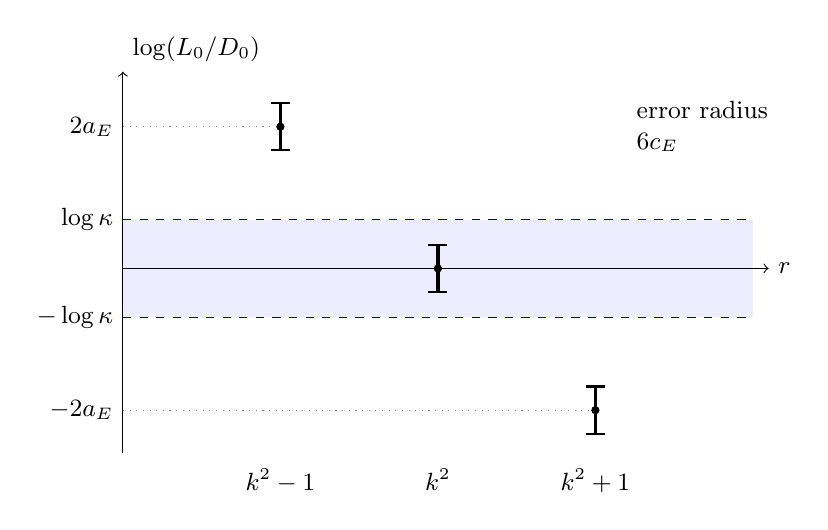
\begin{tikzpicture}[x=1cm,y=1cm,font=\small]
  \fill[blue!7] (1,-.62) rectangle (9,.62);
  \draw[blue!55!black,dashed] (1,.62)--(9,.62);
  \draw[blue!55!black,dashed] (1,-.62)--(9,-.62);
  \draw[->] (1,-2.35)--(1,2.5)
    node[above right] {$\log(L_0/D_0)$};
  \draw[->] (1,0)--(9.2,0) node[right] {$r$};
  \node[left] at (1,.62) {$\log\kappa$};
  \node[left] at (1,-.62) {$-\log\kappa$};
  \draw[gray,dotted] (1,1.8)--(3,1.8);
  \draw[gray,dotted] (1,-1.8)--(7,-1.8);
  \node[left] at (1,1.8) {$2a_E$};
  \node[left] at (1,-1.8) {$-2a_E$};
  \foreach \x/\y in {3/1.8,5/0,7/-1.8}{
    \draw[very thick] (\x,\y-.30)--(\x,\y+.30);
    \draw[thick] (\x-.12,\y-.30)--(\x+.12,\y-.30);
    \draw[thick] (\x-.12,\y+.30)--(\x+.12,\y+.30);
    \fill (\x,\y) circle (1.5pt);
  }
  \node[below] at (3,-2.42) {$k^2-1$};
  \node[below] at (5,-2.42) {$k^2$};
  \node[below] at (7,-2.42) {$k^2+1$};
  \node[right,align=left] at (7.4,1.8) {error radius\\$6c_E$};
\end{tikzpicture}
\caption{The index window, schematically for \(k\ge2\). At index \(r\),
the logarithmic ratio lies within \(6c_E\) of \(2a_E(k^2-r)\).
The choice \(6c_E<\log\kappa<2a_E-6c_E\) puts the entire middle
interval in the admissible band and every other integer-index interval
outside it. The error bars represent bounds, not additional variables.}
\label{fig:height-window}
\end{figure}


The uniqueness assertion includes every intermediate point in every
fixed scalar chain, all six coordinates of each rational code, and every
nested comparison or branch witness. Inactive local tuples are zero.
Appendix~\ref{app:witnesses} specifies the complete tuple and follows it
through the power and computation constructions.

\section{A power graph from a growth function}\label{sec:power}

We now turn the growth function into a single-fold definition of
exponentiation.  The two sides of its growth estimate serve different
purposes.  The upper bound limits the indices of solutions to two Pell
equations, so that congruences determine those indices.  The lower bound
ensures that the intended Pell solutions satisfy the imposed limit.
The use of Pell sequences to recover exponentiation belongs to the
classical Diophantine representation method.  The paired Pell equations,
index congruences, and quotient used here adapt Matiyasevich's exponential
single-fold construction \cite[Section~4]{mati1974}, as presented in
\cite[Section~6, Lemma~6.1 and Theorem~5]{cco2024}.
Our cutoff is supplied by the complete
single-fold polynomial graph of Proposition~\ref{prop:growth}.
We begin with the elementary facts about Pell equations needed for this
argument.

\begin{lemma}\label{lem:pell-sequences}
For an integer $a\ge2$, put $D=a^2-1$ and define integers
$x_i(a),y_i(a)$ by
\[
 (a+\sqrt D)^i=x_i(a)+y_i(a)\sqrt D\qquad(i\ge0).
\]
Every solution in positive integers of $x^2-Dy^2=1$ is
$(x_i(a),y_i(a))$ for exactly one $i\ge1$.  Moreover,
\begin{equation}\label{eq:pell-bounds}
 y_i(a)\equiv i\pmod{a-1},\qquad
 (2a-1)^{i-1}\le y_i(a)\le(2a)^{i-1}\quad(i\ge1).
\end{equation}
If $b,u\ge2$ and $n\ge0$ are integers, then
\begin{equation}\label{eq:pell-ratio}
 b^n\le \frac{y_{n+1}(bu)}{y_{n+1}(u)}
 \le b^n\left(1+\frac1{2u-1}\right)^n.
\end{equation}
\end{lemma}

\begin{proof}
The integer $D$ lies strictly between $(a-1)^2$ and $a^2$, so it is
not a square.  Write $\alpha=a+\sqrt D$.  Its inverse is
$a-\sqrt D$, and both belong to $\ZZ[\sqrt D]$.
Every positive power of $\alpha$ has positive integer coefficients
and norm one.
For any positive solution, $\beta=x+y\sqrt D>1$ has inverse
$x-y\sqrt D>0$.  Choose the unique integer $i\ge0$ for which
\[
 1\le\gamma:=\beta\alpha^{-i}<\alpha.
\]
The coefficients of $\gamma=x'+y'\sqrt D$ are integers and its norm is
one.  If $\gamma>1$, then
\[
 x'=\frac{\gamma+\gamma^{-1}}2>0,\qquad
 y'=\frac{\gamma-\gamma^{-1}}{2\sqrt D}>0.
\]
Thus $y'\ge1$ and $x'^2=1+Dy'^2\ge a^2$, which implies
$\gamma\ge\alpha$, a contradiction.  Consequently $\gamma=1$ and
$\beta=\alpha^i$.  Since $\beta>1$, the index is positive; it is unique
because $\alpha>1$.

Taking coefficients gives
\[
 y_0(a)=0,\quad y_1(a)=1,\quad
 y_{i+2}(a)=2a\,y_{i+1}(a)-y_i(a).
\]
Reduction modulo $a-1$ proves the congruence in
\eqref{eq:pell-bounds} by induction.  For $i\ge1$ define
$R_i(a)=y_{i+1}(a)/y_i(a)$.  The recurrence gives
\[
 R_1(a)=2a,\qquad R_{i+1}(a)=2a-\frac1{R_i(a)}.
\]
Induction therefore yields $2a-1\le R_i(a)\le2a$.  Multiplying these
bounds proves the remaining assertions of \eqref{eq:pell-bounds}.
In particular,
\begin{equation}\label{eq:pell-index-lower}
 y_{n+1}(a)\ge(2a-1)^n\ge n+1\qquad(n\ge0).
\end{equation}

We also have $R_i(bu)\ge bR_i(u)$ for every $i\ge1$.
There is equality for $i=1$, and the induction step follows from
\[
 R_{i+1}(bu)-bR_{i+1}(u)
 =\frac b{R_i(u)}-\frac1{R_i(bu)}\ge0.
\]
On the other hand, the bounds just proved give
\[
 \frac{R_i(bu)}{R_i(u)}\le\frac{2bu}{2u-1}.
\]
Multiplication for $i=1,\ldots,n$ proves \eqref{eq:pell-ratio}.
For $n=0$ both products are empty and $y_1(bu)=y_1(u)=1$,
so the same assertion holds.
\end{proof}

The next proposition uses only the growth estimate and the uniqueness
of the entire witness for its defining system.  In particular, no
monotonicity hypothesis on the growth function is needed.

\begin{proposition}\label{prop:power}
Suppose that $g:\NN\to\NN$ has a complete single-fold graph and that
there are fixed constants $\delta>0$ and $u_0\in\NN$, with $u_0\ge4$,
such that
\begin{equation}\label{eq:power-growth-hypothesis}
 \delta(\log u)^2<\log g(u)<u\log u
 \qquad(u\ge u_0).
\end{equation}
Then the relation
\[
 \Pow(b,n,c)\quad\Longleftrightarrow\quad
 b\ge2\ \hbox{ and }\ c=b^n
 \qquad(b,n,c\in\NN)
\]
has a complete single-fold representation.  In particular, for each
$b\ge2$ and $n\in\NN$, the output $c$ and all auxiliary variables
are jointly unique.
\end{proposition}

\begin{proof}
The ratio in Lemma~\ref{lem:pell-sequences} suggests taking $c$ as the
integer quotient of $y_{n+1}(bu)$ by $y_{n+1}(u)$. To make its error
less than one without introducing a free scale, we prescribe $u$ as a
polynomial in $c,b,n$. Once the cutoff and congruences have fixed both
Pell indices at $n+1$, the lower ratio bound gives $c\ge b^n$, allowing
the factor $c+1$ to control the error. For the intended output $c=b^n$,
a sufficiently large fixed power of $c+1$ also makes $g(u)$ exceed both
intended Pell coordinates.

Choose a fixed positive integer
\begin{equation}\label{eq:power-ell}
 \ell>\frac3{\delta\log2}.
\end{equation}
Use the following finite system, in which all displayed variables are
natural numbers and $v=g(u)$ denotes one call to the given single-fold
system:
\begin{align}
 &b\ge2,\qquad
 u=(c+1)^\ell(n+1)(b+1)+u_0,\qquad v=g(u),
       \label{eq:power-input}\\
 &X^2-\bigl((bu)^2-1\bigr)F^2=1,\qquad
 Y^2-(u^2-1)H^2=1,                         \label{eq:power-pell}\\
 &0<F<v,\qquad 0<H<v,                     \label{eq:power-cutoff}\\
 &F=n+1+(bu-1)q,\qquad H=n+1+(u-1)q',      \label{eq:power-residue}\\
 &F=cH+r,\qquad r<H.                      \label{eq:power-division}
\end{align}
The exponent $\ell$ is fixed, so the formula for $u$ is polynomial.
As in Section~\ref{sec:conventions}, each inequality contributes its
unique slack variable.  The constants in
\eqref{eq:power-growth-hypothesis} determine the choice of $\ell$.
Only the fixed integers $\ell,u_0$ enter the system; $\delta$ and
logarithms occur only in its proof.

\smallskip
\noindent\emph{Every solution has the prescribed output.}
First observe the numerical bound
\begin{equation}\label{eq:pell-index-cutoff}
 u^u<(2u-1)^{u-1}\qquad(u\in\NN,\ u\ge4).
\end{equation}
Indeed, let $f(u)=(2-1/u)^{u-1}/u$.  Then $f(4)=343/256>1$, and
\[
 \frac{f(u+1)}{f(u)}
 =\frac u{u+1}
   \frac{(2-1/(u+1))^u}{(2-1/u)^{u-1}}
 >\frac{2u-1}{u+1}>1\qquad(u\ge4).
\]
This proves \eqref{eq:pell-index-cutoff}.

In a solution to \eqref{eq:power-input}--\eqref{eq:power-division},
$u\ge u_0\ge4$.  The positive coordinates $F,H$ make $X,Y$ positive
as well.  Lemma~\ref{lem:pell-sequences} therefore gives unique
indices $i,j\ge1$ with
\[
 F=y_i(bu),\qquad H=y_j(u).
\]
By \eqref{eq:power-growth-hypothesis} and
\eqref{eq:pell-index-cutoff},
\[
 F,H<v<u^u<(2u-1)^{u-1}.
\]
If either index were at least $u$, the lower bound in
\eqref{eq:pell-bounds} would contradict this strict inequality.
Hence $1\le i,j<u$.

The formula for $u$ also gives $1\le n+1<u-1$.
The congruence for $H$ in \eqref{eq:power-residue} forces
$j\equiv n+1\pmod{u-1}$.  Among $1,\ldots,u-1$ exactly the
integer $n+1$ has that residue.  Similarly,
$i\equiv n+1\pmod{bu-1}$, and both integers lie between $1$ and
$u-1<bu-1$.  Thus
\begin{equation}\label{eq:pinned-pell-indices}
 i=j=n+1.
\end{equation}
We have now determined the two Pell indices.  It remains to identify
the integer quotient imposed by \eqref{eq:power-division}.

By \eqref{eq:pell-ratio},
\[
 b^n\le F/H\le b^n(1+z)^n,
 \qquad z=\frac1{2u-1}.
\]
Since $0\le r<H$, the division equation gives
$c=\lfloor F/H\rfloor\ge b^n$.
We have $nz<1$, and the binomial theorem followed by a geometric
series gives
\[
 (1+z)^n-1
 \le\sum_{h=1}^{n}(nz)^h
 \le\frac{nz}{1-nz}.
\]
This also holds when $n=0$, with an empty sum.  It follows that
\begin{equation}\label{eq:power-quotient-error}
 0\le \frac FH-b^n
 \le\frac{b^n n}{2u-1-n}
 \le\frac{cn}{2u-1-n}<1.
\end{equation}
For the last inequality, the formula for $u$ and $\ell\ge1$ give
$u\ge(c+1)(n+1)+4$, whence
\[
 2u-1-n-cn\ge cn+2c+n+9>0.
\]
The integer quotient is consequently $c=b^n$.

\smallskip
\noindent\emph{The prescribed output has a witness.}
Fix $b\ge2$ and $n\ge0$, set $c=b^n$, and define $u$ by
\eqref{eq:power-input}.  Take the unique output and complete witness
for $v=g(u)$, and put
\[
 \begin{split}
 F=y_{n+1}(bu),&\qquad X=x_{n+1}(bu),\\
 H=y_{n+1}(u),&\qquad Y=x_{n+1}(u).
 \end{split}
\]
These coordinates satisfy the Pell equations.
The congruences in \eqref{eq:pell-bounds}, together with
\eqref{eq:pell-index-lower}, give the nonnegative integer quotients
\[
 q=\frac{F-n-1}{bu-1},\qquad
 q'=\frac{H-n-1}{u-1}.
\]
The ratio estimate and the same calculation as
\eqref{eq:power-quotient-error}, now with $c=b^n$, give
$0\le F/H-c<1$.  Thus $r=F-cH$ is a natural number less than $H$.

We must still check that these particular Pell coordinates lie below
$v$.  From $c=b^n$ and the definition of $u$ we obtain
\[
 \log u\ge\ell n\log b\ge\ell n\log2.
\]
Also $b<u$ and $2<u$, so $\log(2bu)\le3\log u$.
The upper bound in \eqref{eq:pell-bounds} now gives
\begin{equation}\label{eq:power-existence-cutoff}
 \log F\le n\log(2bu)
 \le\frac3{\ell\log2}(\log u)^2
 <\delta(\log u)^2<\log v.
\end{equation}
The same estimate applies to $H$, using
$H\le(2u)^n\le(2bu)^n$.  Hence $0<F,H<v$, as required.
When $n=0$, these statements give explicitly
\[
 c=1,\quad F=H=1,\quad X=bu,\quad Y=u,
 \quad q=q'=r=0;
\]
the strict cutoff still follows from
\eqref{eq:power-existence-cutoff}.

\smallskip
\noindent\emph{The whole witness is unique.}
For fixed $b,n$, the soundness argument first fixes $c$.
The formula in \eqref{eq:power-input} then fixes $u$, after which the
single-fold hypothesis fixes $v$ and every auxiliary variable in its
call.  Equation~\eqref{eq:pinned-pell-indices} fixes $F,H$.
Their Pell equations fix the natural coordinates $X,Y$, since a
nonnegative square root is unique.  The two residue equations fix
$q,q'$, and the division equation fixes $r$.
All inequality slacks are then fixed.  Any variables introduced to
name polynomial arguments are fixed by their defining equalities.
The indices $i,j$ used in the proof introduce no variables in the
system.  Thus the complete tuple is unique.  Finally, the constraint
$b\ge2$ excludes all solutions at $b=0,1$.
\end{proof}

Applying Proposition~\ref{prop:power} to the function supplied by
Proposition~\ref{prop:growth} gives the power graph used in the rest
of the proof.

\section{Testing containment of binary digits}\label{sec:subset}

For $x,y\in\NN$, write $x\bits y$ if every binary digit equal to one
in $x$ is also equal to one in $y$.  More explicitly, if
\[
 x=\sum_{i\ge0}x_i2^i,\qquad y=\sum_{i\ge0}y_i2^i,
 \qquad x_i,y_i\in\{0,1\},
\]
then $x\bits y$ means $x_i\le y_i$ for every $i$.
In particular, $x\bits y$ implies $x\le y$.
We will use this relation to restrict the permitted positions of
nonzero digits in a computation code.  Exponentiation lets us test it
by extracting one digit from a binomial expansion.
Large-base extraction of binomial coefficients goes back to Julia
Robinson \cite[Section~5]{robinson1952}.  Its combination with binomial
parity gives the binary-masking method used by
Jones and Matiyasevich \cite[Section~3]{jm1991}; the parity criterion is
the case modulo two of Lucas's theorem \cite[Section~3, p.~52]{lucas1878}.
We give its short proof and
retain all witnesses of the three power calls and two divisions.

\begin{proposition}\label{prop:subset}
The relation $x\bits y$ on $\NN^2$ has a complete single-fold
Diophantine representation.
\end{proposition}

\begin{proof}
Require $x\le y$ and use three calls to
Proposition~\ref{prop:power} to specify
\begin{equation}\label{eq:subset-powers}
 B=2^{y+1},\qquad H=B^x,\qquad N=(B+1)^y.
\end{equation}
All three bases are at least two.
Introduce natural variables $s,d,r,t$ and impose
\begin{equation}\label{eq:subset-digit}
 N=sBH+dH+r,\qquad d<B,\qquad r<H,\qquad d=2t+1.
\end{equation}
For fixed $B,H,N$, the equation and the two bounds determine
$s,d,r$ uniquely.  Indeed, division of $N$ by $H$ first determines
$r$ and the quotient $sB+d$; division of this quotient by $B$ then
determines $s,d$.

The binomial theorem gives
\[
 N=(B+1)^y=\sum_{j=0}^{y}\binom yj B^j.
\]
Every coefficient is at most $\sum_{j=0}^{y}\binom yj=2^y<B$,
so this is the base-$B$ expansion of $N$ without carries.
As $H=B^x$ and $0\le x\le y$, the digit $d$ extracted in
\eqref{eq:subset-digit} is therefore $\binom yx$.

To determine its parity, work in the polynomial ring over the field
$\mathbb F_2$ with two elements.  Repeated squaring gives
$(1+Z)^{2^i}=1+Z^{2^i}$, and hence
\[
 (1+Z)^y=\prod_{i:\,y_i=1}(1+Z^{2^i})
 \qquad\hbox{in }\mathbb F_2[Z].
\]
Each monomial in the product is obtained by choosing some of the
positions where $y_i=1$.  Uniqueness of binary expansion ensures
that distinct choices have distinct exponents.  The coefficient of
$Z^x$ is thus one precisely when $x\bits y$.
Equivalently, $\binom yx$ is odd precisely in that case.
The final equation $d=2t+1$ in \eqref{eq:subset-digit} proves the
required equivalence.

For a true instance, the three outputs in
\eqref{eq:subset-powers} and all their auxiliary variables are
unique by Proposition~\ref{prop:power}.  The two divisions uniquely
determine $s,d,r$, and oddness uniquely determines the natural number
$t=(d-1)/2$.  Every inequality slack is likewise unique.
Conversely, when the relation is false, either $x>y$ or the extracted
digit is even, so the system has no solution.
The case $x=y=0$ causes no exception: it gives
\[
 B=2,\quad H=N=1,\quad s=r=t=0,\quad d=1.
\]
Thus existence and uniqueness include every natural input pair.
\end{proof}

\section{One witness for a halting computation}\label{sec:computation}

Propositions~\ref{prop:power} and~\ref{prop:subset} provide single-fold
definitions of powers and binary containment. We now use these relations to
encode an entire computation by finitely many natural numbers. Determinism
will determine the computation, and a clock will determine the size of the
blocks used to encode it. Both features are needed: a fixed computation
admits many encodings if its block size is left free.
The method of recording register computations in a large power-of-two
base comes from Jones and Matiyasevich's bit-masking construction
\cite{jm1984}; see especially the exposition in
\cite[Section~4]{jm1991}. Determining the base from the input and
computation time already appears in Chaitin's account
\cite[Sections~2.3 and~2.6]{chaitin1987}. Here a clock and a dyadic
interval determine the base. We verify both the decoding of every
solution and the uniqueness of its complete auxiliary tuple.

\subsection{The machine model}

A counter machine has a finite set of states, a distinguished initial state
$q_*$, a distinguished halt state $h$, and finitely many counters with values
in $\NN$. Every state other than $h$ has exactly one instruction of one of
the following forms:
\begin{itemize}
\item $\operatorname{INC}(j)$: increase counter $j$ by one and go to a
specified state;
\item $\operatorname{TESTDEC}(j)$: if counter $j$ is zero, leave it zero and
go to a specified state; otherwise decrease it by one and go to a second
specified state.
\end{itemize}
The other counters remain unchanged. The halt state has no instruction.
Thus every configuration outside $h$ has exactly one successor. Time counts
individual instructions, including those used to implement a subroutine.
This is the classical counter instruction set of
Minsky~\cite[Theorem~Ia]{minsky1961}; register-machine formulations were
also developed by Shepherdson and Sturgis
\cite[Section~10, Result~10.3]{shepherdson1963}. We include the simulation needed
for the direct tuple inputs used here, so no encoded-input convention is
imported into the lemma.

\begin{lemma}\label{lem:counter-universality}
Let $n\geq 1$ and let $S\subseteq\NN^n$ be recursively enumerable. There
is a counter machine that, when its first $n$ counters are initialized to
$a_1,\ldots,a_n$ and its remaining counters to zero, reaches its halt state
if and only if $\mathbf a\in S$.
\end{lemma}

\begin{proof}
Choose a deterministic Turing machine that accepts precisely the unary
input words
$1^{a_1}\#\cdots1^{a_n}\#$ with $\mathbf a\in S$. Any rejecting terminal
behavior can be replaced by an infinite loop, so only acceptance halts.
We describe a simulation using the two instruction types above.

Store the tape strictly to the left and strictly to the right of the
current cell as two stacks; store the current symbol in the finite
control. Give the finitely many tape symbols distinct digits
$1,\ldots,q$, including a digit for the blank symbol, and put $D=q+1$.
A stack with successive symbols $e_0,e_1,\ldots,e_{m-1}$, starting at its
top, is stored as $\sum_{i<m}e_iD^i$. The empty stack is zero.
Allocate distinct counters for the two stacks, the input coordinates,
a scratch counter, and a counter that is always zero.

To push digit $e$ onto a stack of value $v$, compute $Dv+e$.
Repeatedly decrement the stack counter and, after each successful
decrement, increment the initially zero scratch counter exactly $D$
times. Transfer the scratch counter back by repeated decrements of it
and increments of the stack counter; then perform $e$ increments.
The scratch counter is again zero. All repetitions of a fixed length
are implemented by finitely many states.

To pop a nonempty stack, repeatedly decrement its counter, keeping the
number of successful decrements modulo $D$ in the finite control, and
increment the scratch counter after every $D$ successful decrements.
When the stack counter reaches zero, the scratch counter contains the
quotient by $D$ and the control contains the remainder. Transfer that
quotient back to the stack counter. Its original least significant
digit is nonzero, so the remainder gives the symbol popped. An empty
stack returns a blank and stays empty. Again the scratch counter ends
at zero. Moving the tape head pushes the written current symbol onto
one stack and pops the other. Storing additional blank symbols causes
no difficulty, since each finite computation uses finite stacks.

Initialize the right stack by pushing the input word in reverse: for
$i=n,n-1,\ldots,1$, push $\#$ and then push a $1$ for each successful
decrement of input counter $i$. Pop once to obtain the initial current
symbol; the left stack is empty. A zero test on the counter that is
always zero implements an unconditional jump. Every subroutine uses
finitely many states; duplicating these states supplies its finitely
many required return destinations. This gives a deterministic counter
machine with a sole halt state reached exactly on acceptance.
\end{proof}

Fix such a machine for the remainder of the construction. Write $r$ for
its number of counters and $s$ for its number of states. Its initial
counter values are $d_1,\ldots,d_r$, where each $d_j$ is an input
coordinate or zero. In the proof below it is harmless to allow any fixed
list of such initial values. Put
\begin{equation}\label{eq:machine-C}
 C=1+s+\sum_{j=1}^r d_j.
\end{equation}
The symbol $C$ denotes this expression, not an additional choice.
At time $t$ in any run, counter $j$ has value at most $d_j+t<C+t$,
since an instruction increases a counter by at most one. A clock with
value $C+t$ will therefore give a common bound for the counter values.

Regard an increment instruction as one directed arc, labeled $+j$.
Regard a test-decrement instruction as two directed arcs, labeled
$0j$ and $-j$. Each arc retains its specified destination. Let
$\mathcal A$ be this finite set of arcs, and let
$\mathcal A_j^+$ and $\mathcal A_j^-$ denote those labeled $+j$ and
$-j$, respectively. The halt state has no outgoing arc, and
$|\mathcal A|\leq 2s$.

\subsection{A finite system for the run}

\begin{proposition}\label{prop:machine-compiler}
Fix $n\ge1$ and a deterministic counter machine with finitely many states
and counters, instructions $\operatorname{INC}$ and $\operatorname{TESTDEC}$,
and one halt state. Initialize each counter by a fixed choice of an input
coordinate $a_i$ or zero. There is a finite system of integer polynomial
equations in $a\in\NN^n$ and natural auxiliary variables such that, for
every input $a$, the complete auxiliary tuple has exactly one solution
when the initialized machine halts, and no solution when it does not halt.
\end{proposition}

We first give the system using the single-fold relations $\Pow$ and
$\bits$. Every occurrence is a separate call with fresh auxiliary
variables, as in Section~\ref{sec:conventions}. Inequalities use the unique
slacks from that section. All sets indexing the displayed constraints
are fixed finite sets of states, arcs, or counters.

Introduce natural variables $w,B,b,k,H,J,M$ and require
\begin{align}
 &\Pow(2,w,B),\qquad B=4b,\qquad B>2C,\qquad k>0,
       \qquad\Pow(B,k,H),\label{eq:machine-base}\\
 &BJ=H,\qquad (B-1)M=H-1.\label{eq:machine-geometric}
\end{align}
These equations force
\begin{equation}\label{eq:machine-JM}
 B=2^w,\qquad J=B^{k-1},\qquad M=\sum_{t=0}^{k-1}B^t.
\end{equation}
The intended run has $k$ configurations, at times $0,\ldots,k-1$.
In its base-$B$ encodings, each time occupies one block of $w$ binary
digits. The number $M$ has a single $1$ in the lowest position of each
block.
Multiplication by $B$ shifts each block from time $t$ to time $t+1$.
The transition equations below use this shift to place a selected arc's
destination and its counter update in the next configuration.

For every state $q$, introduce $I_q$ and impose
\begin{equation}\label{eq:machine-state-partition}
 I_q\bits M,\qquad \sum_q I_q=M.
\end{equation}
The intended meaning is that the base-$B$ digit of $I_q$ at time $t$
is one exactly when the machine is in state $q$. For every test state
$q$, introduce $Z_q,N_q,V_q$ and impose
\begin{equation}\label{eq:machine-test-partition}
 Z_q\bits I_q,\qquad N_q\bits I_q,\qquad
 Z_q+N_q=I_q,\qquad Z_q+V_q=M.
\end{equation}
Here $Z_q$ records zero branches, $N_q$ records decrement branches, and
$V_q$ records the complement of the zero-branch times.
Define the arc expression $E_a$ to be $I_q$ for an increment arc from
$q$, and $Z_q$ or $N_q$ for the corresponding arc from a test state $q$.
These are expressions in existing variables. For every state impose
\begin{equation}\label{eq:machine-state-transition}
 I_q=\mathbf 1_{q=q_*}
       +B\sum_{\substack{a\in\mathcal A\\\operatorname{dest}(a)=q}}E_a.
\end{equation}
The coefficient $\mathbf 1_{q=q_*}$ is the fixed integer zero or one.

Counter digits will use only the lowest $w-1$ bits of each block,
so their values lie between zero and $B/2-1=2b-1$.
Reserving the top bit will let the decoding proof exclude signed
carries in the counter updates, which include subtraction.
For each counter $j=1,\ldots,r$, introduce $R_j,\rho_j,\eta_j$ and impose
\begin{align}
 &R_j\bits (2b-1)M,\qquad R_j=\rho_jJ+\eta_j,
       \qquad\eta_j<J,\label{eq:machine-counter-bound}\\
 &R_j=d_j+B\left(R_j-\rho_jJ+
       \sum_{a\in\mathcal A_j^+}E_a-
       \sum_{a\in\mathcal A_j^-}E_a\right).
       \label{eq:machine-counter-transition}
\end{align}
For every test state $q$ operating on counter $j$, additionally require
\begin{equation}\label{eq:machine-zero-test}
 R_j\bits (B-1)V_q.
\end{equation}
The intended base-$B$ digits of $R_j$ are the successive values of the
counter. The quotient $\rho_j$ is its final value. Removing $\rho_jJ$
before multiplying by $B$ makes the recurrence stop at the final time.
The mask $(B-1)V_q$ has a zero block at each time selected by $Z_q$
and has all $w$ binary digits equal to one in every other time block.
Thus the containment condition forces the tested counter to vanish at
the selected times.

Finally introduce $R_0,\rho_0,\eta_0$ for a clock and impose
\begin{align}
 &R_0\bits(2b-1)M,\qquad R_0=\rho_0J+\eta_0,
       \qquad\eta_0<J,\label{eq:machine-clock-bound}\\
 &R_0=C+B(R_0-\rho_0J+M-J),\label{eq:machine-clock-update}\\
 &b\leq\rho_0,\qquad 2\rho_0<B.\label{eq:machine-clock-scale}
\end{align}
Its intended value at time $t$ is $C+t$. The last two inequalities put
its final value in $[B/4,B/2)$; this leaves room for all counter digits
and will select exactly one power-of-two base. We now prove that every
solution has these intended meanings, and that every halting run supplies
a solution.

\begin{proof}[Proof of Proposition~\ref{prop:machine-compiler}]
\emph{States and the final halt.}
Take any solution. Since $B>2C$ and $C\geq 1+s$, we have $B>2s$;
also $B=4b\geq 4$. By \eqref{eq:machine-JM}, binary containment in $M$
means that every base-$B$ digit of $I_q$ is zero or one, with no
nonzero digits outside times $0,\ldots,k-1$. The sum in
\eqref{eq:machine-state-partition} has at most $s<B$ in each digit,
so it has no carries. Thus exactly one state is present at each time.
Similarly, \eqref{eq:machine-test-partition} partitions the times of
each test state into its two branches. Consequently a nonhalt state
has exactly one selected outgoing arc, and the halt state has none.

The digit sums on the right of
\eqref{eq:machine-state-transition} are at most
$|\mathcal A|<B$. Hence those equations also have no carries. They
give state $q_*$ at time zero, and at every later time they give the
destination of the selected arc at the preceding time. The halt mask
has an exact form. Each nonhalt state occurrence selects one arc, so
$\sum_{a\in\mathcal A}E_a=M-I_h$. Summing the state equations gives
\[
 M=1+B(M-I_h),\qquad
 BI_h=1+(B-1)M=H=BJ.
\]
Thus $I_h=J$: the halt state occurs precisely at time $k-1$.
There is exactly one selected arc at each time $t<k-1$, and none
at the final time. This also excludes earlier halts and padded records.

\emph{Counter values and zero tests.}
Since $B=2^w=4b$, the integer
$(2b-1)M=(B/2-1)M$ allows exactly the lowest $w-1$ bits of each
block. Thus we can write uniquely
\begin{equation}\label{eq:machine-counter-digits}
 R_j=\sum_{t=0}^{k-1}r_{j,t}B^t,
 \qquad 0\leq r_{j,t}\leq B/2-1.
\end{equation}
Division by $J=B^{k-1}$ gives $\rho_j=r_{j,k-1}$ and determines
$\eta_j$ uniquely. Let $a_{j,t}$ and $f_{j,t}$ indicate whether the
selected arc at time $t$ increments or decrements counter $j$.
They belong to $\{0,1\}$, never both equal one, and are both zero
at the final time.

Expand \eqref{eq:machine-counter-transition} using these digits.
The coefficient of $B^0$ in the resulting signed sum is
$r_{j,0}-d_j$. For $1\leq t<k$ it is
\begin{equation}\label{eq:machine-signed-coefficient}
 r_{j,t}-r_{j,t-1}-a_{j,t-1}+f_{j,t-1}.
\end{equation}
There are no higher coefficients: the final digit of $R_j$ was
removed, and no final arc was selected. The constant coefficient has
absolute value less than $B$, because $d_j<C<B/2$; every coefficient
in \eqref{eq:machine-signed-coefficient} has absolute value at most
$B/2<B$. An integer sum $\sum_{t=0}^{k-1}c_tB^t=0$ with
$|c_t|<B$ has every $c_t=0$: reduce modulo $B$, use that the only
multiple of $B$ in $(-B,B)$ is zero, divide by $B$, and repeat.
It follows that
\begin{equation}\label{eq:machine-actual-update}
 r_{j,0}=d_j,\qquad
 r_{j,t+1}=r_{j,t}+a_{j,t}-f_{j,t}\quad(0\leq t<k-1).
\end{equation}
This argument rules out borrowing as well as carrying.

Since $Z_q$ selects some of the ones of $M$, the equation
$V_q=M-Z_q$ gives base-$B$ digit zero at its zero-branch times and
one at all other times. Thus $(B-1)V_q$ allows every bit in a block
except at those zero-branch times, where it allows none.
Condition~\eqref{eq:machine-zero-test} forces the tested counter
to be zero whenever the zero branch is selected. On a decrement
branch, \eqref{eq:machine-actual-update} and nonnegativity of the
next digit force the tested counter to be positive. Hence every
test and every update is a valid machine instruction.

\emph{The clock and the block size.}
Apply the same coefficient argument to the clock. In
\eqref{eq:machine-clock-update}, the expression $M-J$ has digit
one exactly at times $t<k-1$. Its digit recurrence is therefore
$r_{0,0}=C$ and $r_{0,t+1}=r_{0,t}+1$. In particular,
\begin{equation}\label{eq:machine-clock-value}
 \rho_0=C+k-1.
\end{equation}
The state and counter arguments show that the encoded configurations
form the actual deterministic run from the specified initialization,
and that it first reaches $h$ at time $k-1$. If the machine does not
halt, no solution exists. If it halts after $T$ instructions, then
$k=T+1$ is forced. Conditions~\eqref{eq:machine-clock-scale} become
\begin{equation}\label{eq:machine-unique-scale}
 2(C+T)<B\leq4(C+T).
\end{equation}
For every positive integer $L$, the interval $(2L,4L]$ contains
exactly one power of two: take the smallest power strictly greater
than $2L$, whose predecessor is at most $2L$. Its successor exceeds
$4L$. Thus \eqref{eq:machine-unique-scale} determines $B$ uniquely,
including when an endpoint is a power of two.

\emph{Existence from a halting run.}
Suppose the initialized machine halts after $T$ instructions. Set
$k=T+1$ and choose the unique power of two $B$ in
\eqref{eq:machine-unique-scale}. Since $C\geq2$, we have $B>4$,
so $B$ is divisible by four. Set $b=B/4$, choose the unique exponent
$w$ with $B=2^w$, set $H=B^k$, and use
\eqref{eq:machine-JM} to define $J,M$.
At time $t\leq T$ each counter has value at most $d_j+t$, because
one instruction increases a counter by at most one. Hence its value
is at most $\sum_jd_j+T<C+T<B/2$. The clock values $C+t$ also
are less than $B/2$. Form $R_j$ and $R_0$ from these digits, and
form the state and branch masks from the actual run.

All state equations follow from the transitions. The zero-test
constraints follow from the zero branches. Summing the actual
counter updates gives \eqref{eq:machine-counter-transition},
with the final digit removed before shifting; summing the clock
updates gives \eqref{eq:machine-clock-update}. The remaining
inequalities follow from \eqref{eq:machine-unique-scale}.
Every power and binary-containment call is true on these arguments
and therefore has its required unique auxiliary tuple.
This also handles $T=0$: then $q_*=h$, $k=1$, $J=M=1$,
all arc masks vanish, and every update sum is empty.

\emph{Uniqueness of the complete tuple.}
In any solution, the deterministic run fixes $T$, every state,
every selected branch, and every counter value. It therefore fixes
$k$; the clock inequalities then fix $B$, and hence $w,b,H,J,M$.
The run fixes all $I_q,Z_q,N_q,R_j,R_0$, while
$V_q=M-Z_q$ fixes every $V_q$. Division by the positive $J$
fixes every $\rho_j,\eta_j$, including the clock pair.
These are all the displayed variables. Each introduced argument
variable is equal to an already determined polynomial expression;
every inequality slack is determined by its endpoints. Finally,
Propositions~\ref{prop:power} and~\ref{prop:subset} determine
all auxiliary variables in every expanded call. Their internal
case selectors and inactive variables are included in that
guarantee. Thus uniqueness holds for the complete tuple, not only
for the numbers recording the run.
\end{proof}

\subsection{The resulting polynomial}

\begin{proof}[Proof of Theorem~\ref{thm:main}]
Given the recursively enumerable set $S\subseteq\NN^n$, choose the
machine of Lemma~\ref{lem:counter-universality} and apply
Proposition~\ref{prop:machine-compiler}. Expand each call to a
single-fold relation into its finite polynomial system, using fresh
auxiliary variables, and expand all inequalities and disjoint cases
according to Section~\ref{sec:conventions}.
The number of equations and variables is finite: the machine is
fixed, its state and counter sets are finite, and each relation call
has a fixed finite definition. The time parameter $k$ is one natural
variable; the digit expansions used in the proof introduce no
additional variables indexed by its value.

Write the resulting integer polynomial equations as
$F_1(\mathbf a,\mathbf z)=\cdots=F_N(\mathbf a,\mathbf z)=0$,
where $\mathbf z$ includes every auxiliary coordinate, and set
\[
 P(\mathbf a,\mathbf z)=\sum_{i=1}^N F_i(\mathbf a,\mathbf z)^2.
\]
On natural tuples, $P=0$ is equivalent to the simultaneous
vanishing of all $F_i$. This operation introduces no variables and
preserves the solution set exactly. By the compiler proposition,
that set has one element when $\mathbf a\in S$ and is empty
otherwise, as asserted.
\end{proof}

\section{Consequences for Diophantine solvability}\label{sec:consequences}

For every finite $n\ge1$ and every recursively enumerable
$S\subseteq\NN^n$, Theorem~\ref{thm:main} also gives a finite-fold
representation: each input has at most one complete witness, and therefore
finitely many. The stronger uniqueness assertion yields the promise
undecidability result stated in the introduction. Its proof specializes one
fixed representing polynomial: the degree and number of variables stay fixed,
while the coefficients vary with the input.

\begin{proof}[Proof of Corollary~\ref{cor:unique-h10}]
Fix a nonrecursive recursively enumerable set $S\subseteq\NN$.
Theorem~\ref{thm:main}, with one parameter, supplies a fixed $m\ge1$ and
a fixed polynomial $P\in\ZZ[A,W_1,\ldots,W_m]$ representing $S$
single-fold. Choose one such $P$, put $D=\max\{1,\deg P\}$, and for
each $a\in\NN$ define
\[
 F_a(W_1,\ldots,W_m)=P(a,W_1,\ldots,W_m).
\]
Every $F_a$ has at most one zero in $\NN^m$, and it has a zero exactly
when $a\in S$. This counts the entire remaining tuple
$(W_1,\ldots,W_m)$, including every subsidiary arithmetic variable.
Specialization introduces no variables and does not increase total degree,
so every $F_a$ satisfies the fixed bounds.

Substitution is computable from the finite coefficient encoding of $P$ and
$a$. Although the proof does not numerically specify $P$, the finite code
of this one fixed polynomial can be hard-coded into a Turing machine. Hence $a\mapsto F_a$ is a computable map of encoded inputs.
A hypothetical algorithm with the stated property, applied to $F_a$, would
therefore decide membership in $S$, a contradiction. Every constructed
input satisfies the promise, so the algorithm's behavior outside it is
irrelevant.
\end{proof}

The bounds in Corollary~\ref{cor:unique-h10} are existential: no numerical
values for them or for the fixed polynomial's coefficients are supplied.
The coefficients of $F_a$, and therefore their input bit lengths, may grow
with $a$. The promise permits both zero and one complete solution; it is not an
exactly-one promise. The corollary makes no claim about analogous uniqueness
promises for solutions over $\ZZ$ or $\QQ$.


\appendix
\section{The rank and torsion of the chosen curve}\label{app:rank-one}

\begin{proof}[Proof of Proposition~\ref{prop:rank-one}]
For \(E:y^2=x^3-25x\), we first prove \([E(\QQ):2E(\QQ)]\le8\), which will force
rank at most one.  We then exhibit a nontorsion point and determine
the full torsion subgroup.  For the rank bound we use the standard
two-isogeny descent \cite[Chapter~III, Example~4.5, and
Chapter~X, Section~4, Example~4.8 and Proposition~4.9]{silverman}, giving the kernel and index
calculations explicitly.  For rational
\(a,b\) with \(b(a^2-4b)\ne0\), write
\[
 E_{a,b}:y^2=x^3+ax^2+bx,\qquad
 b'=a^2-4b,\qquad E'=E_{-2a,b'}.
\]
Both curves are nonsingular.  The following maps, with the exceptional
points \(O\) and \((0,0)\) sent to \(O\), are isogenies:
\begin{align}
 \phi:E_{a,b}&\longrightarrow E',&
 \phi(x,y)&=\left(\frac{y^2}{x^2},
                  y\left(1-\frac b{x^2}\right)\right),
 \label{eq:phi-descent}\\
 \psi:E'&\longrightarrow E_{a,b},&
 \psi(X,Y)&=\left(\frac{Y^2}{4X^2},
                  \frac Y8\left(1-\frac{b'}{X^2}\right)\right).
 \label{eq:psi-descent}
\end{align}
Here are the algebraic and geometric checks needed for this assertion.
For the first map, put \(X=x+a+b/x\).  Substitution gives
\[
 X\bigl((X-a)^2-4b\bigr)
     =y^2\left(1-\frac b{x^2}\right)^2,
\]
which is the target equation.  Applying the same formula to \(E'\)
gives \(E_{4a,16b}\).  The scaling \((x,y)\mapsto(4x,8y)\)
is an isomorphism from \(E_{a,b}\) to \(E_{4a,16b}\);
composing with its inverse gives
\eqref{eq:psi-descent}.

These rational formulas extend over the indicated exceptional points.
At \((0,0)\), the equation
\(y^2=x(b+ax+x^2)\) shows that \(y\) has order one and \(x\)
has order two.  The target coordinates in \eqref{eq:phi-descent}
therefore have poles of orders two and three.  Their ratios \(X/Y\)
and \(1/Y\), which are coordinates in the target chart at infinity,
are regular and vanish there.  At \(O\), the functions \(x,y\)
have poles of orders two and three, and the same argument applies.
Away from these points the formulas are regular.  The argument also
applies to the map from \(E'\), and scaling preserves regularity.
Thus the two maps are nonconstant morphisms preserving the identity;
they are group homomorphisms by the standard isogeny theorem
\cite[Chapter~III, Theorem~4.8]{silverman}.

Write \([c]\) for the class of \(c\in\QQ^*\) in
\(\QQ^*/\QQ^{*2}\).  Define
\[
 \alpha:E_{a,b}(\QQ)\longrightarrow\QQ^*/\QQ^{*2},\qquad
 \alpha(O)=[1],\quad \alpha((0,0))=[b],\quad
 \alpha((x,y))=[x]\quad(x\ne0).
\]
This is a homomorphism.  Indeed, a nonvertical line
\(y=\lambda x+\nu\) meets the cubic, with multiplicity, at roots of
\[
 x^3+(a-\lambda^2)x^2+(b-2\lambda\nu)x-\nu^2.
\]
If \(\nu\ne0\), the product of the three roots is \(\nu^2\).
If \(\nu=0\), the root at \((0,0)\) is simple, since \(b\ne0\),
and the other two roots have product \(b\).  In either case the
product of the three \(\alpha\)-values is trivial.  The third
intersection is the negative of the sum of the first two, and
negation leaves \(\alpha\) unchanged.  Vertical pairs have product
class one; pairs involving \(O\) are immediate.  This also treats
tangencies, with intersection multiplicity understood.

We next prove the exact kernel identity
\begin{equation}\label{eq:descent-kernel}
 \ker\alpha=\psi E'(\QQ).
\end{equation}
An affine image other than \((0,0)\) has square x-coordinate by
\eqref{eq:psi-descent}.  An image equal to \((0,0)\) must have
\(X\ne0\), \(Y=0\), and hence
\(X=a\pm2\sqrt b\).  Such a rational preimage exists exactly
when \(b\) is a rational square; its x-coordinate is nonzero since
\(b'\ne0\).  Thus every image is in the kernel, including the
exceptional points.

Conversely, suppose \(x=s^2\ne0\) for a point \((x,y)\) in
the kernel.  Set
\[
 X=2x+a+2y/s,\qquad Y=2sX.
\]
The product of \(2x+a+2y/s\) and \(2x+a-2y/s\) is \(b'\),
so \(X\ne0\).  The identity
\(X^2-(2a+4x)X+b'=0\) implies
\(Y^2=X^3-2aX^2+b'X\).  Formula~\eqref{eq:psi-descent}
then gives first coordinate \(x\) and second coordinate
\(s(X-b'/X)/4=y\).  When \((0,0)\) is in the kernel, its
preimages were just exhibited; \(O\) is always an image.
This proves \eqref{eq:descent-kernel}.

Let \(\alpha'\) be the analogous squareclass homomorphism on
\(E'\).  Applying the kernel calculation to \(E'\), and using
the scaling above, gives
\(\ker\alpha'=\phi E_{a,b}(\QQ)\).
For \(xy\ne0\), the x-coordinate of \(\psi\phi(x,y)\) is
\[
 \frac{(x^2-b)^2}{4y^2}=x([2](x,y)),
\]
as follows by expanding the usual tangent formula
\(((3x^2+2ax+b)/(2y))^2-a-2x\).
The points therefore agree up to sign.  At \(O\) and the points
with \(y=0\), the composition and doubling both give \(O\).
Since the image of a homomorphism is closed under negation, this
pointwise sign ambiguity still gives
\(\psi\phi E_{a,b}(\QQ)=2E_{a,b}(\QQ)\).
The map induced by \(\psi\) from \(E'(\QQ)/\phi E_{a,b}(\QQ)\)
onto \(\psi E'(\QQ)/2E_{a,b}(\QQ)\) consequently yields
\begin{equation}\label{eq:descent-index}
 [E_{a,b}(\QQ):2E_{a,b}(\QQ)]
 \le |\operatorname{im}\alpha|\,
      |\operatorname{im}\alpha'|.
\end{equation}

The descent has reduced the desired index bound to two squareclass
computations. We now bound those images for our concrete curve;
finite generation will then turn the index bound into a rank bound.
We specialize to \(a=0,b=-25\).  For integral \(a,b\), a
point with \(xy\ne0\) can have an odd valuation in its
x-coordinate only at a prime dividing \(b\).  Write \(v_p(x)\)
for the exponent of the prime \(p\) in the rational number \(x\).
To see the assertion, if
\(v_p(x)<0\), then \(x^2\) is the unique term of smallest
valuation in \(x^2+ax+b\), so
\(2v_p(y)=3v_p(x)\).  If \(v_p(x)>0\) and \(p\nmid b\),
then \(x^2+ax+b\) is a unit, so \(2v_p(y)=v_p(x)\).
In either situation \(v_p(x)\) is even.  Including the
exceptional points, this gives
\[
 \operatorname{im}\alpha\subseteq\{[1],[-1],[5],[-5]\}.
\]
The second curve is \(E':y^2=x^3+100x\).  Every nonzero
x-coordinate on it is positive, and the same valuation argument gives
\[
 \operatorname{im}\alpha'\subseteq\{[1],[2],[5],[10]\}.
\]
Its image does not contain \([2]\).  Otherwise write
\(x=2m^2/e^2\), with nonzero coprime integers \(m,e\).
Substitution gives
\[
 \left(\frac{ye^3}{2m}\right)^2=2m^4+50e^4=N^2
\]
for an integer \(N\), because a rational number with integral
square is integral.  Reduction modulo five first forces
\(5\mid m,N\).  Writing \(m=5m_1\), \(N=5N_1\) then gives
\[
 N_1^2=50m_1^4+2e^4,
\]
which is again impossible modulo five, since \(5\nmid e\).
A subgroup of the four displayed squareclasses that omits \([2]\)
has size at most two.  Thus \eqref{eq:descent-index} gives
\([E(\QQ):2E(\QQ)]\le8\).

By the Mordell--Weil theorem, \(E(\QQ)\) is finitely generated
\cite[Chapter~VIII, Theorem~4.1]{silverman}.  If its rank is \(r\)
and its finite torsion subgroup is \(\mathcal T\), then
\[
 [E(\QQ):2E(\QQ)]
   =2^r|\mathcal T/2\mathcal T|
   =2^r|\mathcal T[2]|=2^{r+2},
\]
since its rational points of order dividing two are precisely
\(O,(0,0),(5,0),(-5,0)\).  Hence \(r\le1\).
The point \((-4,6)\) is nontorsion: the Nagell--Lutz theorem
for an integral short Weierstrass equation \(y^2=x^3+Ax+B\)
says that a nonidentity
rational torsion point has integral coordinates and either
\([2]Q=O\) or \(y(Q)^2\mid4A^3+27B^2\)
\cite[Chapter~VIII, Corollary~7.2]{silverman}.
Here \(36\nmid62500\), so the rank is one.

The same theorem determines the torsion completely.  For integral
coordinates on our curve, reduction modulo three gives
\(y^2\equiv x^3-x\equiv0\), so \(3\mid y\).
A torsion point with \(y\ne0\) would also satisfy
\(y^2\mid62500\), a contradiction.  Thus every affine torsion
point has \(y=0\), giving the claimed list.  Finally choose a
point \(P\) whose image generates the infinite cyclic quotient
\(E(\QQ)/\mathcal T\).  Its cosets, and then the torsion
translates within each coset, give the asserted unique expression.
\end{proof}

\section{The complete auxiliary tuple}\label{app:witnesses}

This appendix fixes one finite expansion of the systems used in the proof.
Its purpose is to make explicit which coordinates the single-fold assertion
counts. Each call has a fresh internal tuple. Its displayed output is
counted by its caller, and its displayed inputs are already available.
Equal-valued coordinates in distinct calls remain distinct variables.
Every coordinate below ranges over \(\NN\).

\paragraph{Primitive conventions.}
A polynomial equality introduces no auxiliary variable. A weak comparison
\(F\ge G\) introduces the single slack \(F-G\); a strict comparison
\(F>G\) introduces \(F-G-1\). Naming a polynomial expression introduces
one variable with its defining equality. Rational comparisons first clear
their positive denominators, so their slacks are integer differences.
For a disjoint case construction,
include every Boolean selector, every local guard slack, and every
coordinate of every local call. Multiply all local equations by the case
selector and set all local coordinates to zero when that case is inactive.
These rules apply recursively to nested calls. In particular, a zeroed
inactive rational code has no ungated positive-denominator requirement.

\paragraph{Rational and point arithmetic.}
The six coordinates of a rational code are
\((p,n,d,t,s,q)\) from \eqref{eq:rational-code}: the two sign parts,
positive denominator, inverse residue, its interval slack, and the inverse
quotient. A point has its identity flag and both complete rational codes.
For an addition, the caller counts the output point once. The internal
addition tuple consists of seven selectors, four local
six-coordinate slope codes (Cases 3, 4, 6, and 7), and the four strict
comparison slacks in those cases. Other guards are equalities and require
no further witnesses. Clearing denominators introduces no free multiplier.
A maximum uses two selectors and one local comparison slack in each case;
the first case receives a tie. All inactive local coordinates are zero.

Fix one addition chain for \([m_*]Q\) once and for all; for example, use
\(Q,2Q,\ldots,m_*Q\). Each addition contributes its output point and the
internal addition tuple just described. A height call \(W(Q)\) has one
displayed height output, counted by its caller. Its internal tuple contains
the scalar chain and the maximum tuple applied to the final x-coordinate's
absolute numerator and denominator. The chain length is a fixed constant.

\paragraph{The growth graph.}
For a representative test on a point \(Q\), retain its height output
\(h_Q\), the internal height tuple, the four codes of \(Q+t\) and their
addition tuples, and six comparison slacks: one for \(y(Q)\ge0\), one for
\(h_Q>1\), and four for \(x(Q)\ge x(Q+t)\). Affineness is a flag equation.
This test has unique internal witnesses for a fixed representative; the
bracket and window are what fix the representative itself.

Write \(\xi\) for the entire internal tuple of a call \(v=g(u)\).
It consists of the following blocks:
\begin{itemize}
\item The codes of \(Q,R\) and both representative-test tuples, including
      their height outputs \(h_Q,h_R\).
\item The codes of \(Q+P,Q-P,R+P,R-P,[2]Q\), all five addition tuples,
      and their five height outputs with five complete internal height tuples.
\item The two neighbor-height maxima with both complete maximum tuples,
      and \(L_0,D_0\) with their product equalities.
\item The four slacks in the bracket and window: if the neighbor maxima
      are \(N_Q,N_R\), these are
      \[
       u+W_1-h_Q,\quad N_Q-u-W_1-1,\quad
       \kappa D_0-L_0,\quad \kappa L_0-D_0.
      \]
\end{itemize}
Impose \(v=h_R\). Here the already present internal coordinate \(h_R\)
and the displayed output \(v\) are distinct variables fixed to the same
value. The heights \(h_Q,h_R\) are reused in the products and inequalities.
All signs, denominators, slopes, selectors, and scalar-chain points remain
inside \(\xi\). The integer indices \(k,r\) and the real quantities in
the growth proof are not variables of this tuple.

\paragraph{Powers and binary containment.}
For displayed arguments \((b,n,c)\), one complete internal power tuple is
\[
 (u,v,X,Y,F,H,q,q',r,\sigma_b,\sigma_F,\sigma_{Fv},
       \sigma_H,\sigma_{Hv},\sigma_r,\xi),
\]
where the six slacks, in order, have values
\[
 b-2,\quad F-1,\quad v-F-1,\quad
 H-1,\quad v-H-1,\quad H-r-1.
\]
The output \(c\) is counted by the caller. No sign variable accompanies
the natural square roots \(X,Y\); no Pell index is quantified.

For a binary-containment call on \((x,y)\), name \(e=y+1\) and
\(A=B+1\). Include
\[
 (e,A,B,H,N,s,d,r,t,\sigma_{xy},\sigma_d,\sigma_r)
\]
and three separate complete internal power tuples for
\(\Pow(2,e,B)\), \(\Pow(B,x,H)\), and \(\Pow(A,y,N)\).
The three slacks are \(y-x,B-d-1,H-r-1\). The quotients and remainders
are precisely \(s,d,r\), and the parity quotient is \(t\).
These calls, including all of their growth tuples, remain present when
\(x=0\) or \(y=0\).

\paragraph{The computation tuple.}
Let the fixed machine have \(s\) states, \(r\) counters, and
\(\tau\) test states. Enumerate each of these finite sets once.
The displayed machine coordinates are
\[
 (w,B,b,k,H,J,M),\qquad
 (I_q)_q,\qquad (Z_q,N_q,V_q)_{q\text{ a test state}},
 \qquad (R_j,\rho_j,\eta_j)_{0\le j\le r}.
\]
Include the \(r+5\) comparison slacks
\[
 B-2C-1,\quad k-1,\quad (J-\eta_j-1)_{0\le j\le r},
 \quad \rho_0-b,\quad B-2\rho_0-1.
\]
Name \(D=(2b-1)M\) and, for each test state, \(D_q=(B-1)V_q\),
using their defining equalities. Include the two internal power tuples
for \(\Pow(2,w,B)\) and \(\Pow(B,k,H)\). Finally include a complete
binary-containment tuple for each of
\[
 \begin{gathered}
  I_q\bits M,\qquad Z_q\bits I_q,\qquad N_q\bits I_q,\\
  R_j\bits D\quad(0\le j\le r),\qquad
  R_{j(q)}\bits D_q\quad(q\text{ a test state}),
 \end{gathered}
\]
where \(j(q)\) is the counter tested at \(q\). There are
\(s+3\tau+r+1\) such calls. Arc masks are expressions in the displayed
state and test masks and introduce no variables. The expression
\(C=1+s+\sum_jd_j\) also introduces no variable.

This is a finite recursive specification of the whole auxiliary tuple.
Its length depends only on the fixed machine and fixed arithmetic
constructions, not on an input or its halting time. Proof digits,
configurations, and time indices are not extra coordinates.
The computation proof fixes the actual run first, then its base,
then every displayed value above. The preceding graphs fix all their
internal coordinates, including every inactive branch. Replacing the
resulting finite list of equations by its sum of squares introduces no
coordinate and preserves exactly this complete tuple.

\bibliographystyle{plain}
\bibliography{references}
\end{document}
